\documentclass[conference]{IEEEtran}
\IEEEoverridecommandlockouts
% The preceding line is only needed to identify funding in the first footnote. If that is unneeded, please comment it out.
\usepackage[backend=biber,style=ieee]{biblatex}
\usepackage {hyperref}
\usepackage{amsmath,amssymb,amsfonts}
\usepackage{algorithmic}
\usepackage{graphicx}
\usepackage{textcomp}
\usepackage{changepage}
\usepackage{xcolor}
\usepackage{array,tabularx}
\def\BibTeX{{\rm B\kern-.05em{\sc i\kern-.025em b}\kern-.08em
    T\kern-.1667em\lower.7ex\hbox{E}\kern-.125emX}}
%Adjustments to tabularx
\renewcommand{\tabularxcolumn}[1]{m{#1}}
\newcolumntype{Y}{>{\raggedright\arraybackslash}X}
    

\bibliography{false_feature_rejection.bib}
\begin{document}

\title{NCT Project: Detector and Discriptor Outlier Rejection Evaluation for SLAM in MIS\\
}

\author{\IEEEauthorblockN{1\textsuperscript{st} Nicolas Schmitt}
\IEEEauthorblockA{
Technische Universität Dresden \\
Dresden, Germany}
\and
\IEEEauthorblockN{2\textsuperscript{nd} Boyang Liu}
\IEEEauthorblockA{
Technische Universität Dresden \\
Dresden, Germany}
\and
\IEEEauthorblockN{3\textsuperscript{rd} Florian Thiessenhusen}
\IEEEauthorblockA{
Technische Universität Dresden \\
Dresden, Germany}
}

\maketitle

\begin{abstract}
\end{abstract}

\section{Introduction}
Performing Simultaneous Localization and Mapping (SLAM) inside the human body for Minimally Invasive Surgery (MIS) can be a difficult task due to the challenging environment. \\
One part of executing a feature-based SLAM is the detection and matching of such feature points. Finding those points usually works well in well lit and rigid environments, where the object of interest is not near the camera. As these conditions are not met under MIS conditions with deforming tissue and homogeneous surfaces, the tracking of features becomes harder. \cite{chen_slam_2019} \\
In this paper, we present different feature detection and outlier rejection methods that might improve the quality of the matching results. 

% Example Section
\section{Example Picture}
Fig.~\ref{tree}

\begin{figure}[htbp]
\centerline{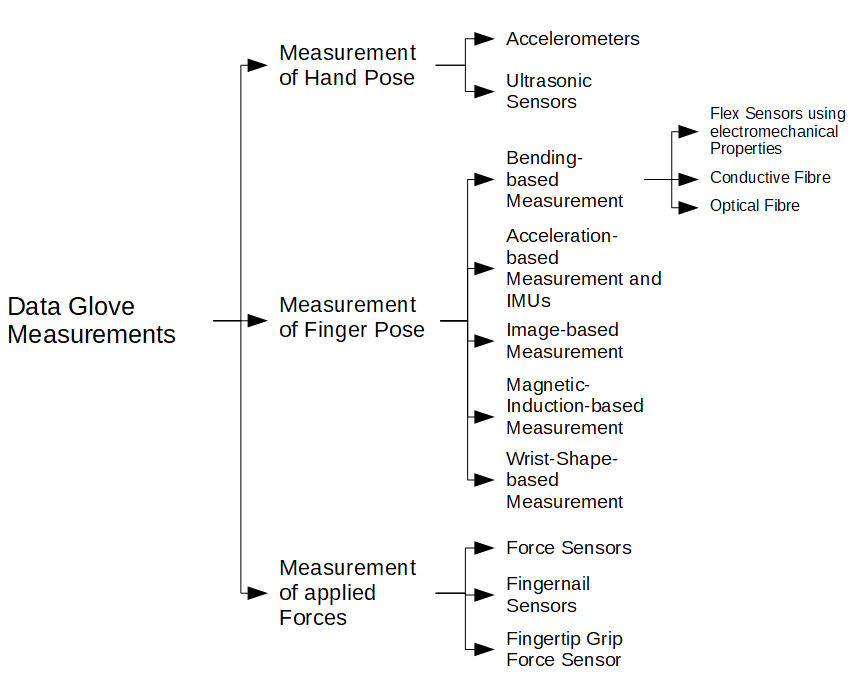
\includegraphics[width = 8.5cm]{Pictures/Tree.png}}
\caption{Arrangement of measurement systems in a tree structure.}
\label{tree}
\end{figure}

\begin{table}[htbp]
\caption{Example Table}
\begin{center}
\begin{tabularx}{\linewidth}{|Y|Y|Y|}
\hline
\textbf{Measurement System}&\textbf{Advanteges}&\textbf{Disadvanteges} \\
\hline
Accelerometers & no line of sight needed & wrong orientation of sensors can cause false measurements \\
\hline
Ultrasonic Sensors & direct position measurement, no error propagation & requires line of sight and special measurement environment  \\
\hline

\end{tabularx}
\label{tab1}
\end{center}
\end{table}
%Example Section End

\section{Conclusion} 


\AtNextBibliography{\small}
\printbibliography
\end{document}
